\section{Introduction}
\label{chapter:intro}

\subsection{Quark Gluon Plasma}

\subsubsection{Fundamental particles}

Over the history of physics, people were fascinated with discovering new fundamental building blocks of matter. The definition of fundamental particles changes as the scientific knowledge evolves. As the energy of the probe increases, the scale of matter we could observe becomes smaller. Everyday matter is composed of atoms (meaning "unable to cut" in Greek), once was thought to be matter's elementary particles in the 1910s. This view changed when subatomic constituents of the atom were identified. In the 1930s, the electron and the proton had been observed, along with the photon, the mediator binds the nuclei and electron. That was when Quantum Electrodynamics (QED) began to develop, which describes how light interact with matter and is the first theory where full agreement between quantum mechanics and special relativity is achieved.

Proton, neutron and electron were considered as the fundamental particles for a long time, until 1968. Deep Inelastic Scattering (DIS) experiment at SLAC showed that the proton contained much smaller, point-like objects. This experiment confirmed the quark model proposed a few years earlier, in which quarks interact with each other through mediator named as gluon. Color charge, together with existing basic quantum numbers, was introduced to quarks to make the new experimental observations fit into Pauli exclusion principle. Color can be interpreted as an analog of electric charge in the QED. The theory of the strong interaction between quarks and gluons is known as Quantum Chromodynamics (QCD). The QCD exhibits two unique properties, color confinement and asymptotic freedom, which we will discuss in Section~\ref{sec:color_confinement}.

The standard model is the theoretical framework describing all the currently know elementary particles. This model contains six flavors of quarks, named up (u), down (d), strange (s), charm (c), bottom (b) and top (t). Antiparticles of quarks are called antiquarks, which have the same mass and spin, but opposite electric and color charges. The whole family of fundamental particles are shown in the Figure~\ref{fig:intro_standard_model}, where particles related to weak interaction are not discussed.

\begin{figure}[H]
\centering
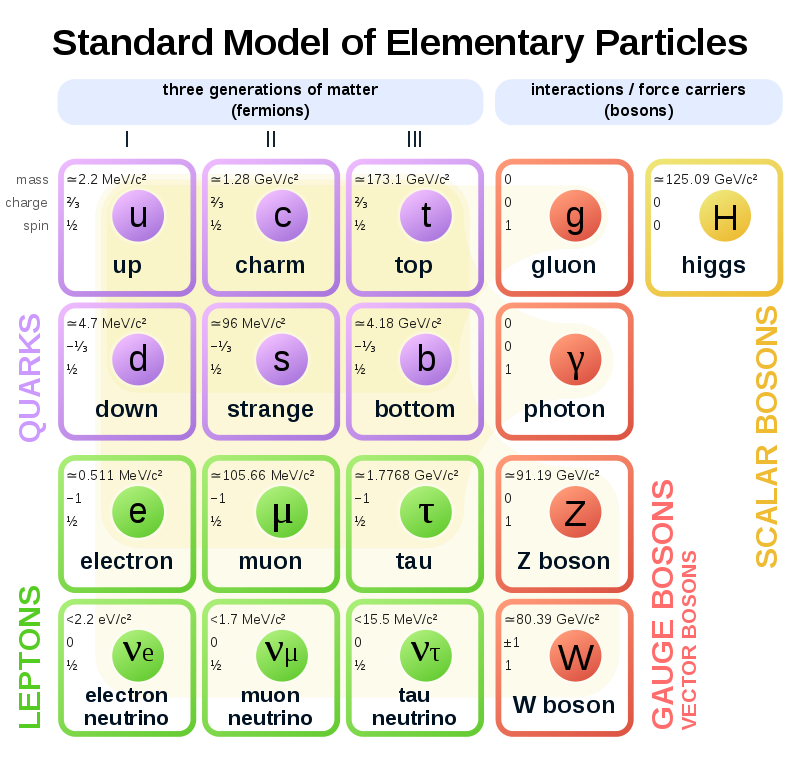
\includegraphics[width=.95\linewidth]{figs/chapter_intro/standard_model.png}
\caption{Standard model of fundamental particles. Each of the first three columns forms a generation of matter. The figure is taken from Ref.~\cite{wiki:standard_model}.}
\label{fig:intro_standard_model}
\end{figure}



\subsubsection{Color confinement}
\label{sec:color_confinement}

In QCD, color confinement is the phenomenon that color charged particles (quarks and gluons) cannot be isolated, and therefor cannot be directly observed under normal conditions. This means that quarks and gluons must clump together to form hadrons. The two main types of hadrons are the baryons (three quarks) and mesons (one quark, one antiquark). In addition, colorless glueball formed only of gluons are also consistent with color confinement, though difficult to identify experimentally.

The origin of color confinement lies within one feature of QCD: asymptotic freedom. Unlike QED, where the electric field interaction becomes stronger as the energy scale decreases, asymptotic freedom is a property of some gauge theories that causes interactions between particles to become asymptotically weaker as the energy scale increases and the corresponding length scale decreases. This phenomenon can be understood qualitatively by noting that the force-carrying gluons of QCD have color charge, unlike the photons of QED. Whereas the electric field between electrically charged particles decrease rapidly as those particles are separated, the gluon field between a pair of color charges forms a narrow flux (or string) between them. Because of this behavior of the gluon field, the strong force between the particles is constant regardless of their separation.

Therefore, as two quarks are separated, the energy increases, and at some point it becomes energetically favorable for a new quark-anti-quark pair to appear, rather than extending the string further. As a result of this, when quarks are produced in particle accelerators, instead of seeing the individual quarks in detectors, we observe jets of many color neutral particles clustered together. This process is called hadronization, fragmentation or string melting. As a conclusion, free strongly-interaction quarks can not be produced under normal conditions.



\subsubsection{QCD phase diagram}

Due to color confinement, no ``free'' quarks can be found in the hadronic matter. However, with finite spatial extension, concept of hadronic matter appears to lose its meaning at sufficiently high density. At low density, particular quark in a hadron ``knows'' its partner quark. However, at high density, when hadrons start to interpenetrate each other, a particular quark will not be able to identify the quark which was its partner at lower density~\cite{Chaudhuri:2012yt}. Effectively, once we have a system of mutually interpenetrating hadrons, where each quark finds a number of quarks in its vicinity, quarks behave just like they are ``free''. Similar phenomena can happen at high temperature. As the temperature of a nuclear matter is increased, more and more low mass hadrons will be created. The system again will be dense enough and hadrons will start to interpenetrate. It is customary to call this quark matter as QGP, which is a thermalized state of quarks and gluons, where quarks and gluons are free to move in a nuclear volume rather than a nucleonic volume. Even though the explanation above is over-simplified and on the conceptual level, it still illustrates an idea why QGP only exists in high density and temperature environment.

The phase diagram of quark matter is not well known, either experimentally or theoretically. A commonly conjectured form of phase diagram is shown in the Figure~\ref{fig:intro_QCD_diagram}, as a function of temperature $T$ and baryon chemical potential $\mu_B$. The solid line represents a first order transition which separates hadronic and QGP phase. The end point of this line is the Critical End Point (CEP). The dashed line at small $\mu_B$ indicates a cross-over transition between the QGP and hadronic phases.

\begin{figure}[H]
\centering
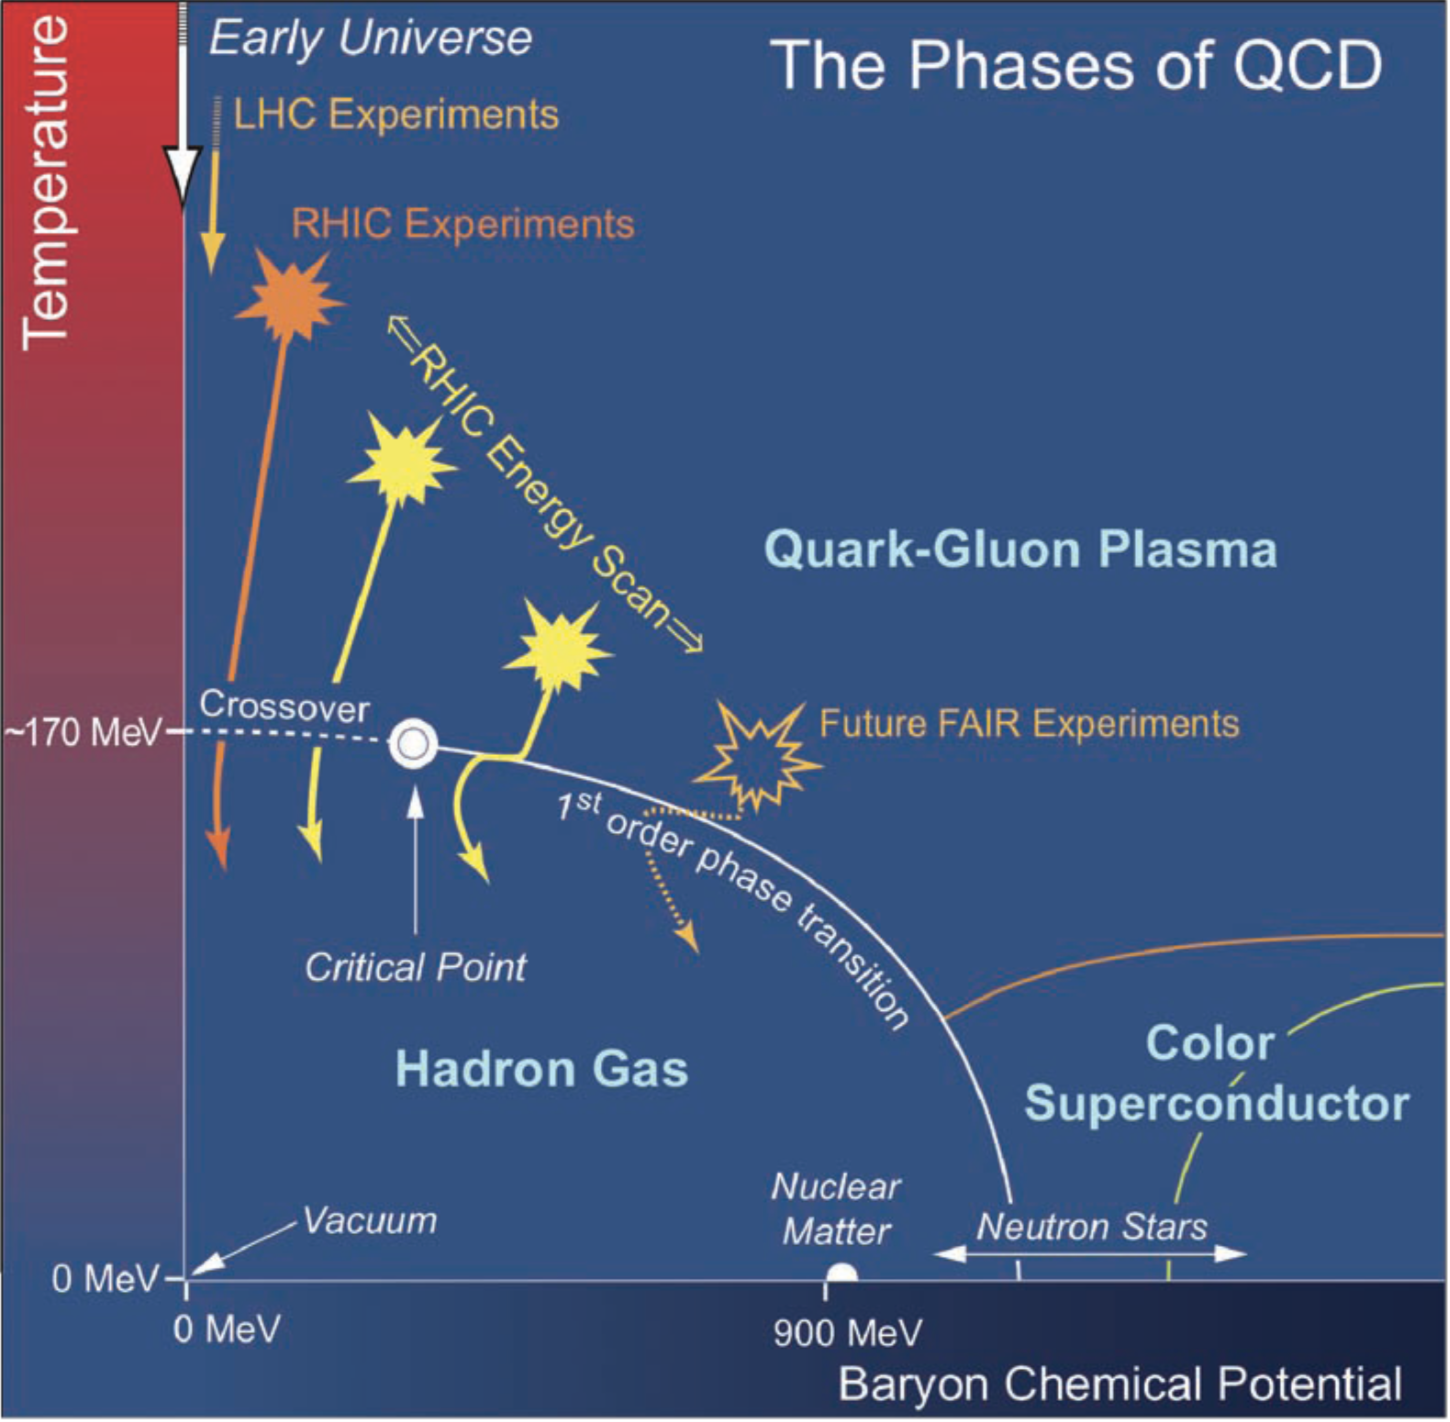
\includegraphics[width=.6\linewidth]{figs/chapter_intro/QCD_diagram.png}
\caption{Schematic QCD phase diagram for nuclear matter. The solid lines show the phase boundaries for the indicated phases. The solid circle depicts the critical point. Possible trajectories for systems created in the QGP phase at different accelerator facilities are also shown.}
\label{fig:intro_QCD_diagram}
\end{figure}

Theoretically, there are several approaches to locate the QCD phase transition boundary. Lattice QCD~\cite{Gupta:1997nd} (LQCD) is a well-established non-perturbative approach formulated on a grid or lattice of points in space and time. LQCD is favored because analytic or pertubative solutions in low-energy QCD are hard or impossible to obtain due to the high non-linear nature of the strong force and the large coupling constant at low energies. However, numerical LQCD calculations can be extremely computationally intensive, and currently there is no formulation of LQCD that allows us to simulate real-time dynamics of QGP. Another independent approach is to incorporate the QCD Lagrangian into MC models such as PYTHIA and HIJING. The results from these models provide important references for comparisons between models and experiments. We will follow this second approach in this dissertation.



\subsubsection{QGP in cosmology}

Why is QGP important to study? For a complete review, refer to Ref.~\cite{Busza:2018rrf}. In the early universe, when dense and temperature are very high, QGP is presumed to be existed. The timeline of big bang can be described as follows:
\begin{itemize}
\item At the earliest time, temperature is at the order of Planck scale temperature. At this stage, quantum gravity is important. String theorists are putting enormous efforts trying to understand this stage.
\item At the later stage of evolution, it is the grand unification scale. Strong and electroweak interactions are unified at this sale. The universe at this scale may also be supersymmetric, where each fermion a boson exists and vice-versa.
\item As the universe further expands and cools, strong and electroweak interactions are separated. At this lower temperature (100 GeV), electroweak symmetry breaks and Baryon asymmetry may be produced. Universe exists as QGP.
\item As temperature approaches 100 MeV, deconfinement-confinement transition occur, and hadrons are formed. All heavy-ion collisions are designed to study matter around this temperature.
\item At temperature 1 MeV, nucleosynthesis starts and light elements are formed. This temperature range is also well studied in nuclear physics experiments.
\item At temperature 1 eV, universe changes from ionised gas to a gas of neutral atoms and structures begin to form.
\end{itemize}

QGP may also exist at the core of a neutron star. Since the radius of neutron star is $\sim 10$ km, but very dense (10 times normal nuclear matter density), at such high density matter is likely to be in the form of QGP. The major difference between QGP at the early universe and that in neutron star is the temperature: at the core of the neutron star it is cold QGP with $T\sim 0$ MeV.



\subsubsection{QGP in heavy ion collision}
\label{sec:qgp_in_lab}

To achieve the high density and temperature for the generation of QGP in lab, over the past 15 years, scientists have been conducting Heavy Ion (HI) experiments by colliding nucleus with high energy. The evolution of HI collisions partially follows several stages of the early universe, and is illustrated in Figure~\ref{fig:intro_QGP_evolution}. In experiments, it is important to understand the evolution of HI collisions since we do not have direct access to the QGP itself. By measuring final stage particles and modeling initial conditions provide important constraints to the properties of QGP.

\begin{figure}[H]
\centering
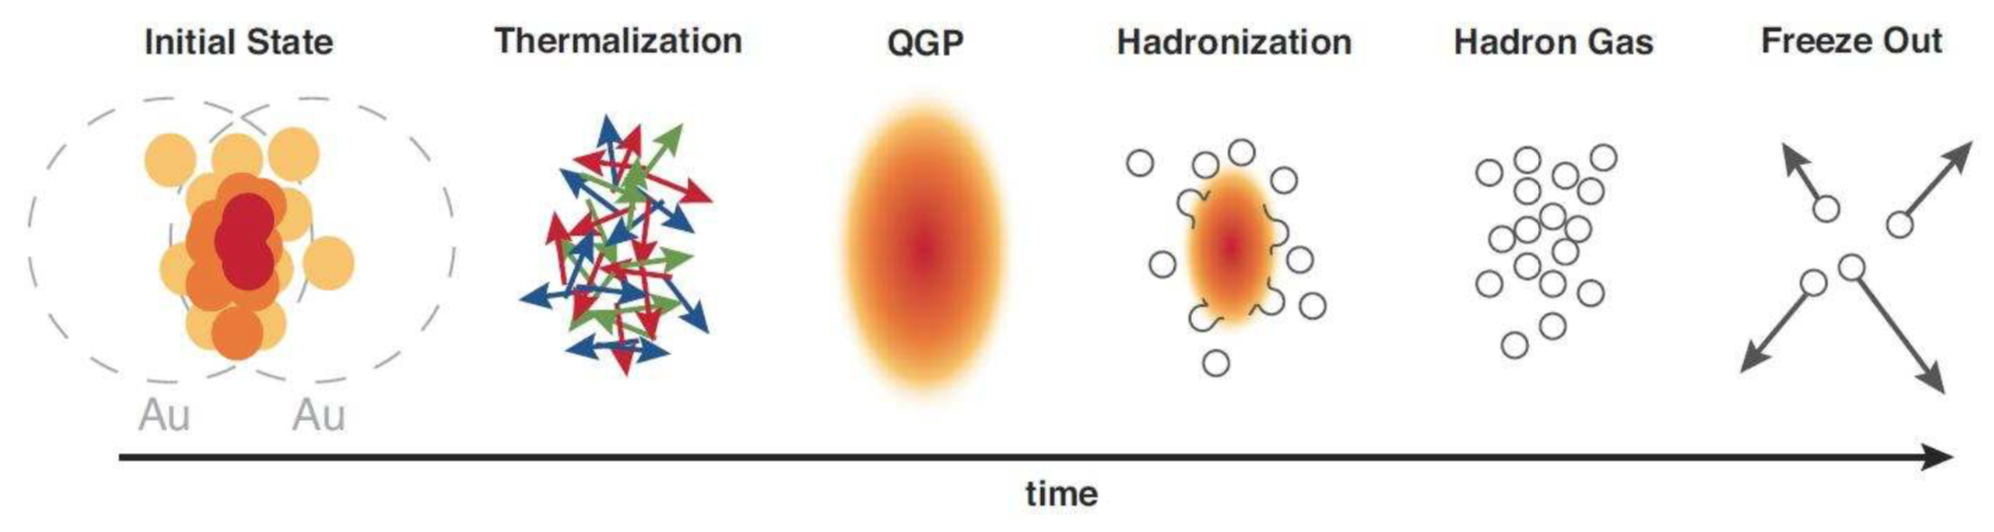
\includegraphics[width=.95\linewidth]{figs/chapter_intro/QGP_evolution.png}
\caption{Schematic illustration of the evolution of nuclear matter created in HI collision. The figure is taken from M. McCumber's PhD thesis.}
\label{fig:intro_QGP_evolution}
\end{figure}

Each stage in the HI collision is briefly discussed as follows:
\begin{itemize}
\item Initial state: in relativistic HI collisions, due to Lorentz contraction, nucleus appear to be "pancake" shape in the lab frame. Participating nucleons collide, generate entropy and produce a nuclear matter with non-uniform energy density. Such non-uniform geometry shape is an important feature for flow measurement, and can be described in two prevailing models: Glauber~\cite{Glauber:1955qq} and Color Glass Condensate (CGC)~\cite{Kharzeev:2002ei}. We will discuss Glauber model in details in Section~\ref{sec:glauber_model}.
\item Thermalization: participating quarks and gluons interact among each other and the system approaches thermal equilibrium. The thermalization time is approximately $\leq 1$ fm/c, a very rapid thermalization as suggested by hydrodynamic calculations~\cite{Adare:2009qk}.
\item QGP: the dense and equilibrated QGP is formed, which then continues to expand and cool down.
\item Hadronization: as the QGP expands, the energy density and temperature decrease, partons begin to form into bound state, i.e. hadrons. This process is named as "recombination" or "coalescence"~\cite{Fries:2008hs}. As discussed above, fragmentation is another different mechanism for partons to hadronize.
\item Hadron gas: at this stage, newly produced hadrons are weakly coupled and still exhibit collective behavior and the whole system is still in equilibrium. The system resembles a dilute gas and can be described by the transport models. Studies showed that the lifetime of this stage is so small that its influence is very limited~\cite{Afanasiev:2007tv}.
\item Freeze out: as the system keeps expanding and diluting, local thermal equilibrium breaks and interactions among hadrons are negligible. Finally the particles stop interact and are observed by the detectors.
\end{itemize}

HI physicists developed different observables that are sensitive to different stages of the HI evolutions, which are summarized in Section~\ref{sec:probing_qgp}, after we introduce the kinematics in HI collision.



\subsection{Kinematics of HI collisions}

To make this dissertation self-consistent, we will introduce kinematics of HI collisions~\cite{Chaudhuri:2012yt}. In relativistic nucleus-nucleus collisions, since the nucleus in the initial stage and particles particles from the final stage travel at the speed close to light, it is convenient to use kinematic variables which take simple form under Lorentz transformation, after changing the frame of reference. In this section, we will first briefly introduce the Lorentz transformation, then discuss several key kinematics frequently used in HI collisions.



\subsubsection{Lorentz transformation}

If $x^\mu$ is the coordinate in one frame of reference, then in another frame of reference the coordinates $x'^{\mu}$ must satisfy:
\begin{equation}
g_{\mu\nu} dx'^\mu dx'^\nu = g_{\mu\nu} dx^\mu dx^\nu
\end{equation}
where Einstein's summation convention is used. $g_{\mu\nu}$ is called the space-time metric:
\begin{equation}
g_{\mu\nu} \equiv diag(1, -1, -1, -1),
\end{equation}
and the natural units $c=1$ is assumed:

In other words, the Lorentz transformation keeps the space-time distance invariant under the transformation. It also has one special property that the speed of light is same in the two frame of reference.

A general Lorentz transformation consists of rotation and translation. Lorentz transformation without rotation is called Lorentz boost. For example, consider the Lorentz boost along the $z$ direction by velocity $\beta$. The transformation can then be written as:
\begin{equation}
\begin{bmatrix}
t' \\
z'
\end{bmatrix}
=
\begin{bmatrix}
\gamma & -\beta\gamma \\
-\beta\gamma & \gamma
\end{bmatrix}
\begin{bmatrix}
t \\
z
\end{bmatrix}
\end{equation}
where $\gamma = 1/\sqrt{1-\beta^2}$ is the Lorentz factor.



\subsubsection{Rapidity variable}

In relativistic energy, rapidity is defined as:
\begin{equation}
\begin{split}
y &= \frac{1}{2} \ln \frac{E+p_z}{E-p_z} \\
&= \tanh^{-1}(\beta_L)
\end{split}
\end{equation}
where $\beta_L = p_z / E$ is called the longitudinal velocity. Rapidity has the advantage over $\beta_L$ that they are additive under a longitudinal boost: a particle with rapidity $y$ in a give frame has rapidity $y + dy$ in a frame which moves relative to the first frame with rapidity $dy$ in the $-z$ direction. This is because the relativistic velocity $\beta_1$ and $\beta_2$ fulfill the addition formula:
\begin{equation}
\beta = \frac{\beta_1 + \beta_2}{1 + \beta_1 \beta_2},
\end{equation}
which is exactly the addition formula for hyperbolic tangents:
\begin{equation}
\tanh (y_1 + y_2) = \frac{\tanh(y_1) + \tanh(y_2)}{1 + \tanh(y_1)\tanh(y_2)}.
\end{equation}

Rapidity is the relativistic analog of non-relativistic velocity. In the non-relativistic limit $p \ll m$, rapidity can be written as:
\begin{equation}
\begin{split}
y &= \frac{1}{2} \ln \frac{\sqrt{p^2 + m^2} + mv_z}{\sqrt{p^2 + m^2} - mv_z} \\
&= \frac{1}{2} [\ln(1+v_z) - \ln(1-v_z)] \\
&\approx v_z
\end{split}
\end{equation}

In terms of the rapidity variables, particle 4-momentum can be parameterized as:
\begin{equation}
p^\mu = (E, p_x, p_y, p_z) = (m_T \cosh y, p_x, p_y, m_T \sinh y)
\end{equation}
with transverse mass $m_T \equiv \sqrt{m^2 + \pT^2} = \sqrt{m^2 + p_x^2 + p_y^2}$.



\subsubsection{Pseudorapidity variable}

For a particle emitted at an angle $\theta$ with respect to the beam axis, rapidity variable can be written as:
\begin{equation}
\begin{split}
y &= \frac{1}{2} \ln \frac{E + p_z}{E - p_z} \\
&= \frac{1}{2} \ln \frac{\sqrt{m^2 + p^2} + p\cos\theta}{\sqrt{m^2 + p^2} - p\cos\theta}
\end{split}
\end{equation}

At very high energy, we have $p \gg m$, and the mass term can be neglected:
\begin{equation}
\begin{split}
y &= \frac{1}{2} \frac{p + p\cos\theta}{p - p\cos\theta} \\
&= - \ln \frac{\theta}{2} \\
&\equiv \eta,
\end{split}
\end{equation}
where $\eta$ is called pseudorapidity. Only angle $\theta$ determine the pseudorapidity. It is a very convenient parameter for experimentalists since details of particles, like mass and full momentum, are not known. While angle of emission $\theta$ can be easily measured experimentally.



\subsubsection{Invariant distribution}

In experiment, one key observable is the distribution of final stage particles. We will construct a Lorentz boost invariant observable that is related to particle distribution.

The differential of Lorentz boost in longitudinal direction is:
\begin{equation}
\begin{split}
dp'_z &= \gamma (dp_z - \beta E) = \gamma (dp_z - \beta \frac{p_z dp_z}{E}) \\
&= \frac{dp_z}{E}\gamma(E - \beta p_z) = \frac{dp_z}{E} E',
\end{split}
\end{equation}
where $EdE = p_z dp_z$ has been used. This means $dp_z / E$ is Lorentz invariant. Since $\pT$ is also Lorentz invariant, $d^3p / E$ is Lorentz invariant.

Then we can construct the Lorentz invariant differential yield:
\begin{equation}
E\frac{d^3 N}{d^3 p} = E\frac{d^3 N}{d^2 \pT dp_z} = \frac{d^3 N}{d^2 \pT dy},
\end{equation}
where the relation $dp_z / E = dy$ is used. Some times experimental results are given in terms of pseudorapidity. The transformation from $(y, \pT)$ to $(\eta, \pT)$ is written as follows:
\begin{equation}
\frac{d^3 N}{d\eta d\pT} = \sqrt{1 - \frac{m^2}{m^2_T \cosh^2 y}}\frac{d^3 N}{dy d\pT}
\end{equation}



\subsubsection{Luminosity}

The luminosity is an important parameter in collider experiments. The reaction rate in a collider is given by:
\begin{equation}
R = \sigma L,
\end{equation}
where $\sigma$ is the interaction cross section and $L$ is the luminosity, in the unit of $\text{cm}^{-2}\text{s}^{-1}$. The luminosity is defined as:
\begin{equation}
L = f n \frac{N_1 N_2}{A},
\end{equation}
where:
\begin{itemize}
\item $f$: revolution frequency
\item $N_1$: number of particles in bunch 1
\item $N_2$: number of particles in bunch 2
\item $n$: number of bunches in one beam in the storage ring
\item $A$: cross-sectional area of the beams
\end{itemize}



\subsubsection{Collision geometry}

In HI collisions, since the number of nucleons is large, nucleus can be approximated as a round shape, as shown in Figure~\ref{fig:intro_HI_geometry}. The impact parameter $b$ is defined as the distance between the centers of nucleus. Due to the elliptic shape of the overlapping region, different kinds of planes can be defined:
\begin{itemize}
\item Reaction Plane (RP): supported by the vector of impact parameter and the beam direction;
\item Participant Plane (PP): supported by the average vector of participants and the beam direction;
\item Event Plane (EP): supported by the average vector of final particles and the beam direction.
\end{itemize}
The reaction and participant planes are defined in the initial stage, thus cannot be measured in experiment directly. While the event plane is one of the key observables in flow analysis.

\begin{figure}[H]
\centering
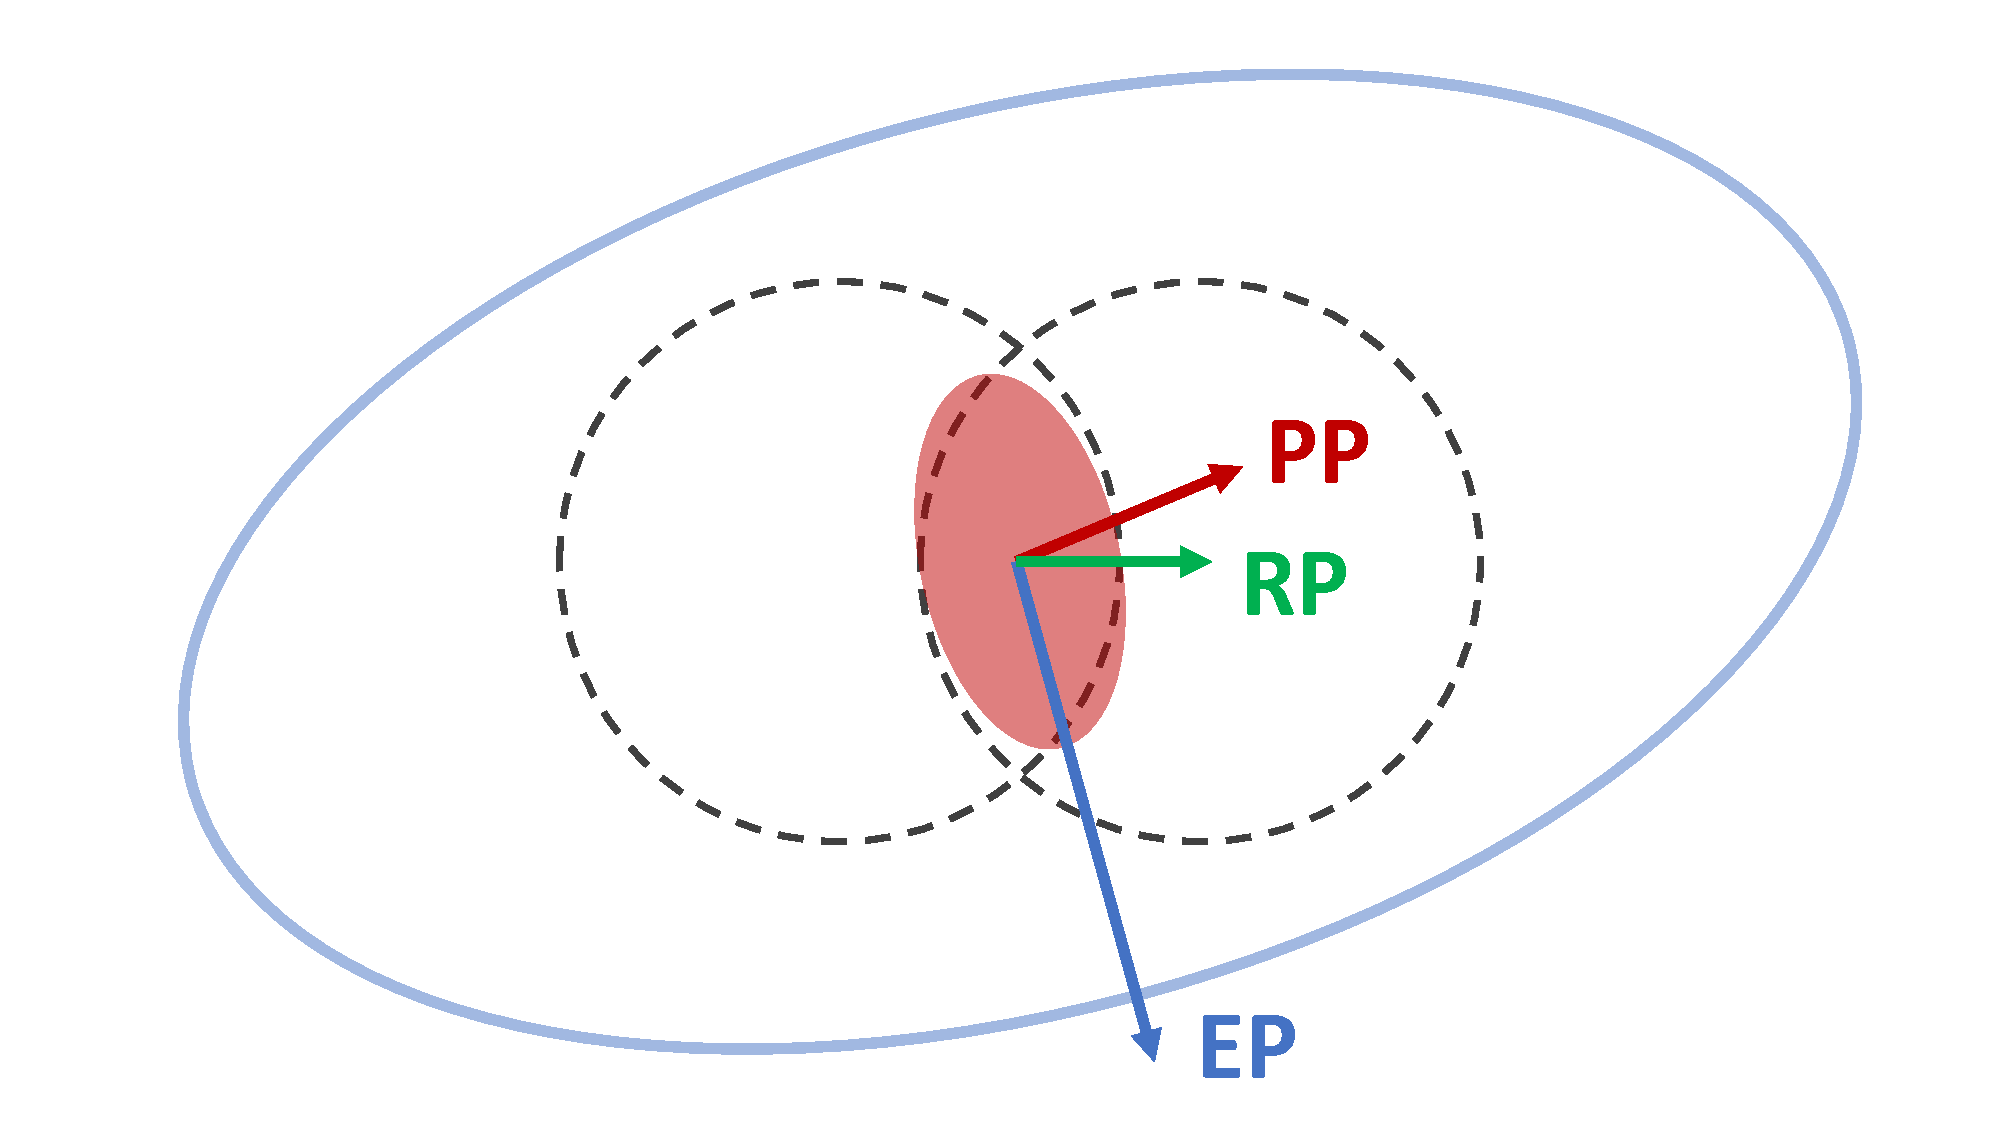
\includegraphics[width=.7\linewidth]{figs/chapter_intro/HI_geometry}
\caption{The definitions of the Reaction Plane (RP), Participant Plane (PP) and Event Plane (EP).}
\label{fig:intro_HI_geometry}
\end{figure}

The particle azimuthal distribution measured with respect to the event plane is not isotropic, and it is conventional to expand it in a Fourier series:
\begin{equation}
E \frac{d^3 N}{d^3 p} = \frac{1}{2\pi} \frac{d^2 N}{\pT d\pT dy}[1+\sum_{n=1} 2 v_n \cos (n(\phi-\Psi))]
\end{equation}
where $\Psi$ is the azimuthal angle of event plane. Note that the left part of the equation is boost invariant. The flow harmonics $v_n$ can be calculated as:
\begin{equation}
v_n = \lr{\cos (n(\phi - \Psi))}
\end{equation}
where the angle brackets mean an average over all particles in all events. Flow coefficients are used for a quantitative characterization of the event anisotropy. The sine term are not present because of the symmetric with respect to the reaction plane.



\subsubsection{Centrality}

Depending upon the impact parameter of the collision, several types of collisions can be defined:
\begin{itemize}
\item Central collision: two nuclei collide head on;
\item Peripheral collision: only glancing interaction between two nuclei.
\end{itemize}
One could image the system created in a central collision can be very different different from that created in a peripheral collision, thus it is crucial to study the observables as a function of impact parameter. Impact parameter of a collision can not be measured experimentally, however, one can have an one-to-one correspondence between impact parameter and some experimental observable. In practice, particle multiplicity $\Nch$ and transverse energy $\Et$ are used since they are monotonic functions of impact parameter. In other cases, by utilizing the detector very far away from the collision point, energy of the spectators can also be an anti-correlated proxy for the impact parameter. See Section~\ref{sec:zero_degree_calorimeter} for details.

The grouping of the events can be done quantitatively. Define a minimum bias collision where all possible collisions are allowed. Figure~\ref{fig:intro_HI_centrality} illustrates how centrality is defined. In this example, distribution of charged particle multiplicity $\Nch$ from $|\eta|<1$ in a minimum bias collision is cut into successive intervals starting from maximum value of multiplicity. First $5\%$ of the high $\Nch$ events corresponds to the top $5\%$ or $0-5\%$ collision centrality. Similarly, centrality class can be defined by measuring the transverse energy.

\begin{figure}[H]
\centering
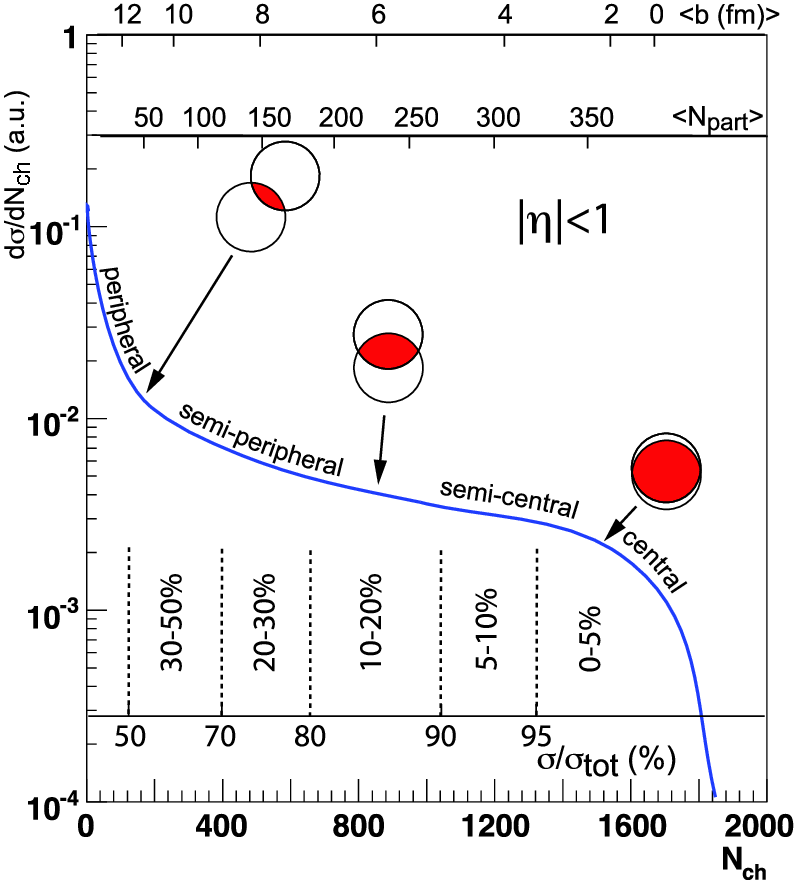
\includegraphics[width=.5\linewidth]{figs/chapter_intro/HI_centrality.png}
\caption{The correlation between the number of participating nucleons in a heavy-ion collision, their cross section and the impact parameter $b$, defining the centrality classes. This figure is taken from Ref.~\cite{Betz:2009jw}.}
\label{fig:intro_HI_centrality}
\end{figure}

Instead of impact parameter, one often defines centrality in terms of number of participating nucleons $N_\text{part}$ (as shown in Figure~\ref{fig:intro_HI_centrality}) or in terms of binary nucleon collision number. These measures have one-to-one relationship with impact parameter and can be calculated in any initial stage models, like Glauber model.



\subsection{Examples of QGP probes}
\label{sec:probing_qgp}

As discussed in Section~\ref{sec:qgp_in_lab}, experimentally it is not possible to probe the QGP directly. In this section, we will present an overview of several major experimental observables that are used to probe the existence and properties of QGP.

\subsubsection{Strangeness production}

The study of the properties of QGP can be undertaken using quarks not present in daily matter observed around us. The experimental and theoretical work relies on the idea of strangeness enhancement. Unlike the up and down quarks, strange quarks are not brought into the reaction by the colliding nuclei. Therefore, any strange quarks or antiquarks observed in experiments have been made from the kinetic energy of colliding nuclei. Furthermore, the mass of strange quarks and antiquarks is equivalent to the temperature or energy at which protons, neutrons and other hadrons dissolve into quarks. This means that the abundance of strange quarks is sensitive to the conditions, structure and dynamics of the deconfined matter phase, and if their number is large it can be assumed that deconfinement conditions were reached.

Strange quarks are naturally radioactive and decay by weak interactions into lighter quarks on a timescale that is extremely long compared with the nuclear-collision time. This makes it relatively easy to detect strange particles through the tracks left by their decay products. Measurement of abundant formation of $K_S^0$, $\Lambda$, $\Xi$ and $\Omega$ as well as their antiparticles is an important observation claiming that QGP has been formed. This abundant formation is often presented in comparison with the scaled expectation from normal proton-proton collisions.

In Figure~\ref{fig:intro_strangeness_ALICE}, the ratios of the yields of $K_S^0$, $\Lambda$, $\Xi$ and $\Omega$ to the pion $(\pi^+ + \pi^-)$ yield as a function of $\lr{d\Nch / d\eta}$ are compared to $p$+Pb and Pb+Pb results at the LHC~\cite{ALICE:2017jyt}. A significant enhancement of strange to non-strange hadron production is observed with increasing particle multiplicity in $pp$ collision. The behavior observed in $pp$ collisions resembles that of $p$+Pb collisions at a slightly lower center-of-mass energy, in terms of both the values of the ratios and their evolution with multiplicity. At high multiplicity, the yield ratios reach values similar to the ones observed in Pb+Pb collisions, where no significant change with multiplicity is observed beyond an initial slight rises. For a more complete review on strangeness enhancement, refer to Ref.~\cite{Koch:2017pda}.

\begin{figure}[H]
\centering
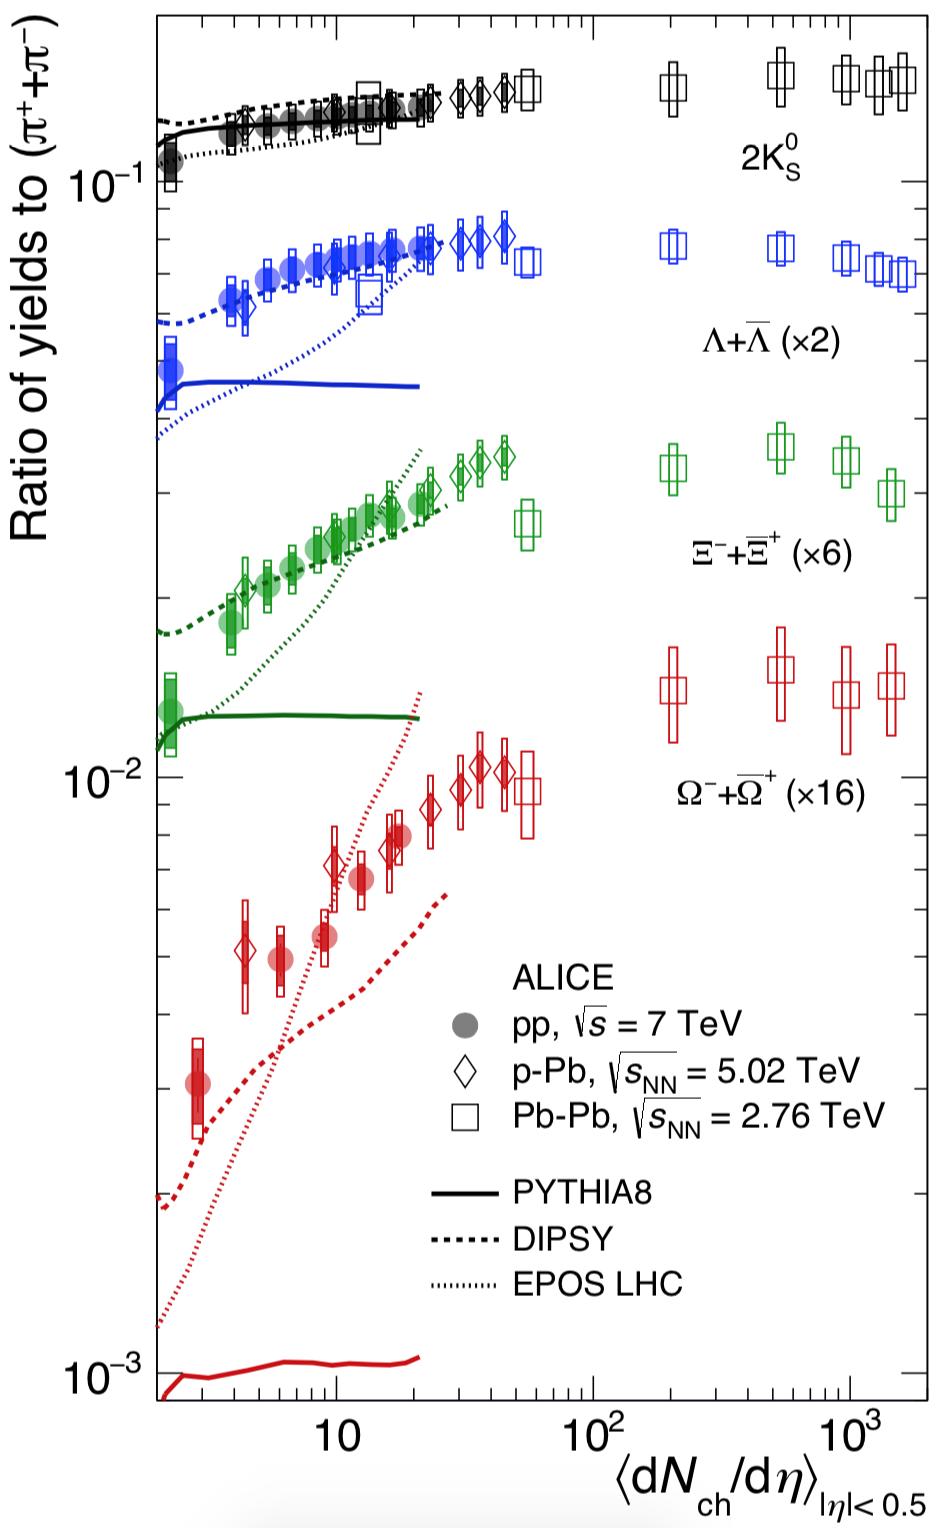
\includegraphics[width=.5\linewidth]{figs/chapter_intro/strangeness_ALICE.png}
\caption{$\pT$ integrated yield ratios to pions as a function of $\lr{d\Nch / d\eta}$ measured in $|y|<0.5$. The values are compared to calculations from MC models and to results obtained in $p$+Pb and Pb+Pb collisions at the LHC. This figure is taken from Ref.~\cite{ALICE:2017jyt}.}
\label{fig:intro_strangeness_ALICE}
\end{figure}



\subsubsection{Elliptic flow}

Elliptic flow describes the azimuthal momentum space anisotropy of particle emission from non-central HI collisions in the plane transverse to the beam direction, and is defined as the second harmonic coefficient of the azimuthal Fourier decomposition of the momentum distribution. Elliptic flow is a fundamental observable since it directly reflects the initial spatial anisotropy, of the nuclear overlap region in the transverse plane, directly translated into the observed momentum distribution of identified particles. Since the spatial anisotropy is largest at the beginning of the evolution, elliptic flow is especially sensitive to the early stages of system evolution. With absence of QGP, distribution of free-streaming particle will be uniform in the transverse direction, thus elliptic flow is strong evidence for the existence of QGP. The focus of this dissertation will be on elliptic flow and we will extend the discussions in Section~\ref{sec:transverse_measurements}.

Figure~\ref{fig:intro_v2_ALICE} presents the comparison of the fully $\pT$ integrated $v_2$ measured in the $20-30\%$ centrality in Pb+Pb collisions with results at lower energies~\cite{Adam:2016izf}. A continuous increase of anisotropic flow for this centrality has been observed from SPS/RHIC to LHC energies. For these fully $\pT$ integrated coefficients, an increase of $5\%$ is observed going from $\sqrt{s_\text{NN}}=2.76$ to 5.02 TeV, which is close to values of the hydrodynamic calculations. For a complete review on collective flow and hydrodynamics, refer to Ref.~\cite{Heinz:2013th, Jeon:2015dfa}.

\begin{figure}[H]
\centering
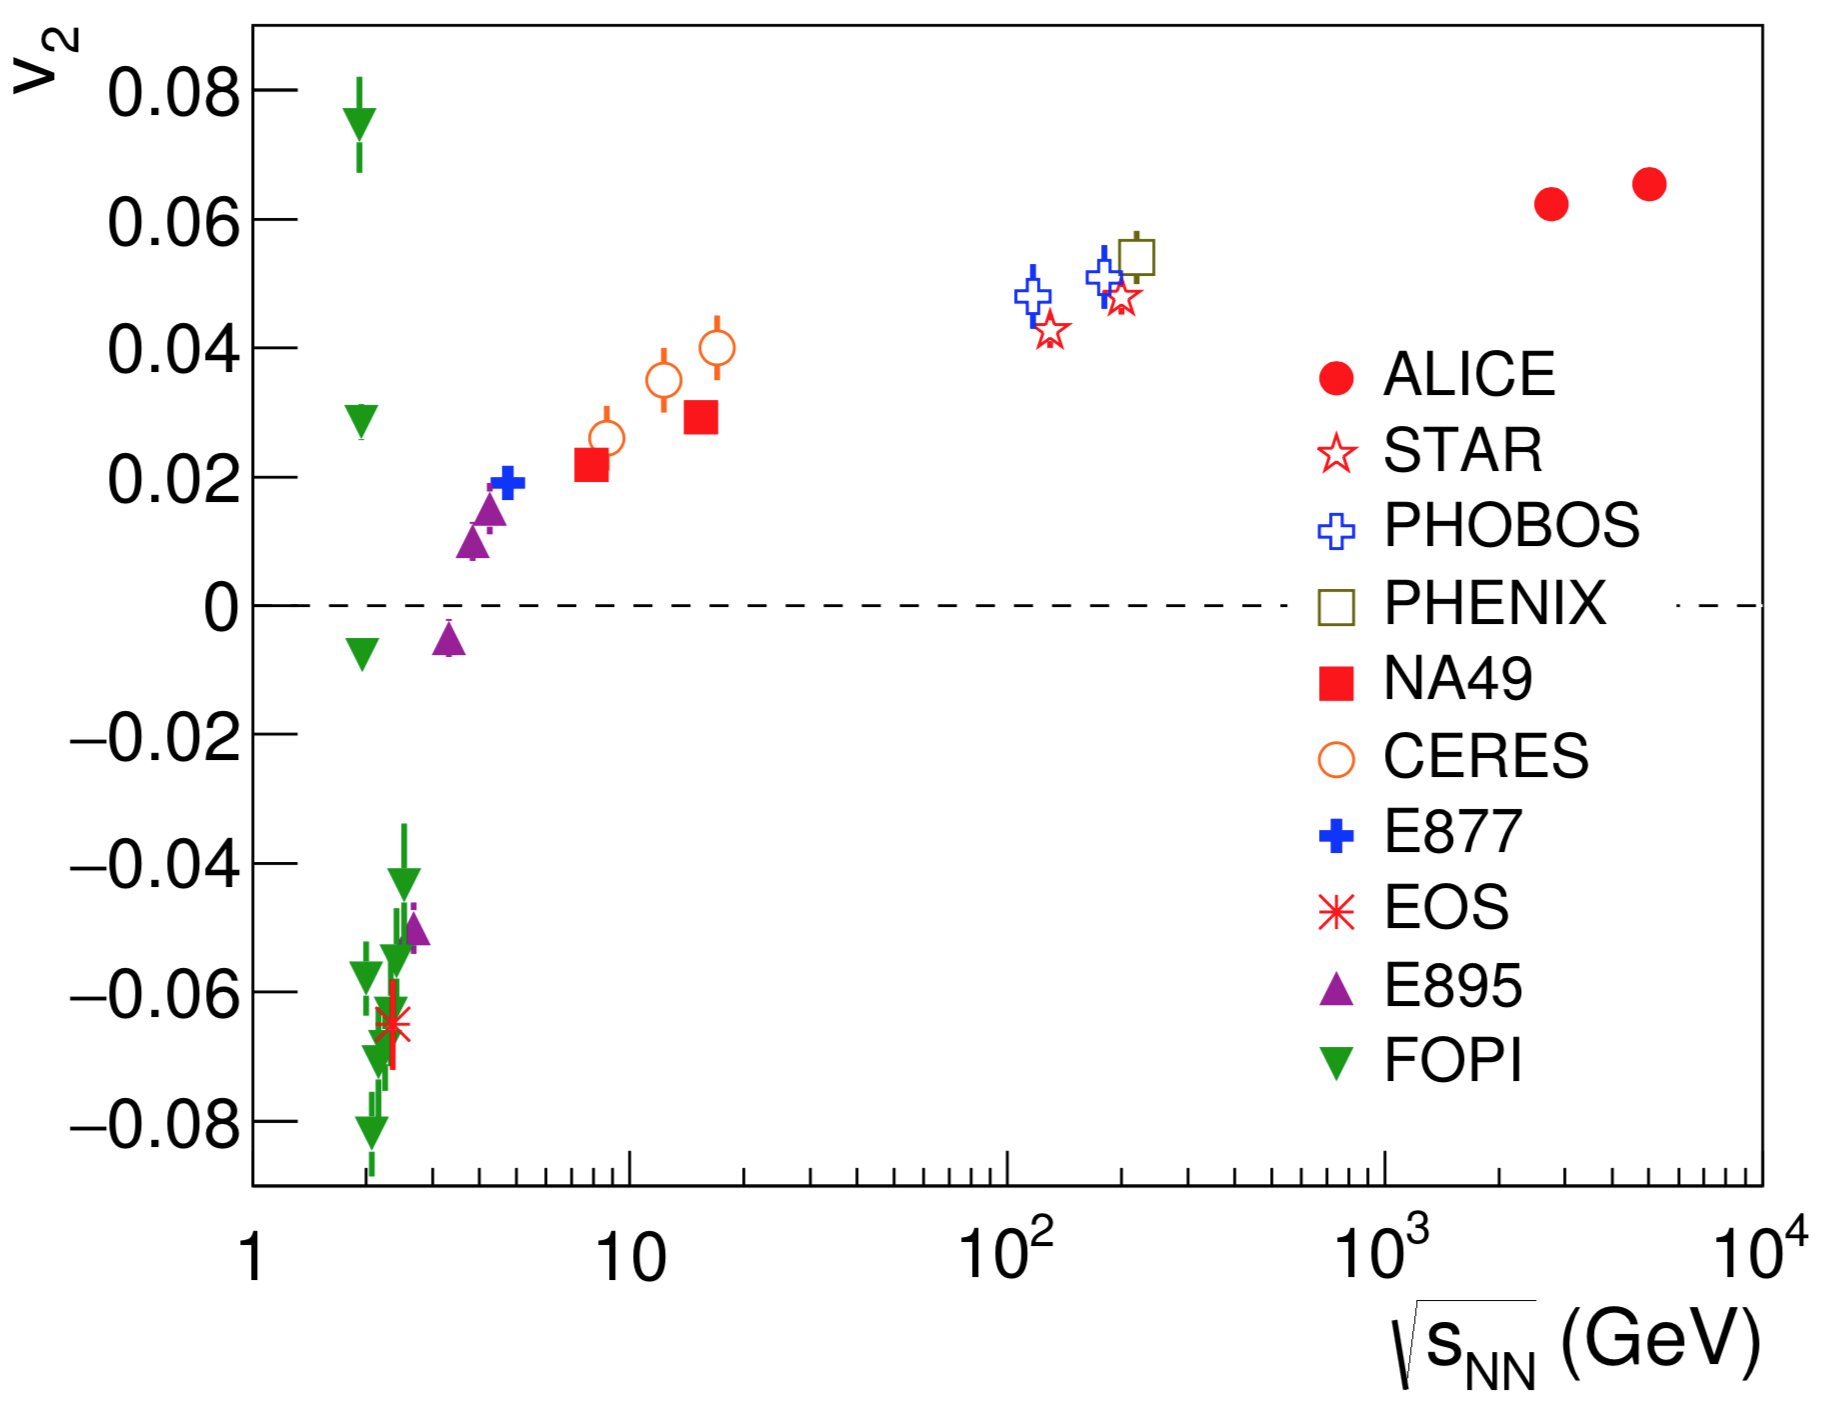
\includegraphics[width=.6\linewidth]{figs/chapter_intro/v2_ALICE.png}
\caption{Integrated elliptic flow $v_2\{4\}$ for the $20-30\%$ most central Pb+Pb collisions at $\sqrt{s_\text{NN}}=5.02$ TeV compared with $v_2$ measurements at lower energies with similar centralities. This figure is taken from Ref.~\cite{Adam:2016izf}.}
\label{fig:intro_v2_ALICE}
\end{figure}



\subsubsection{Jet quenching}

QCD jet produced from early stage collisions of beam quarks and gluons from two nuclei play an essential role in studying transport properties of the QGP produced in these energetic collisions~\cite{Qin:2015srf}. During their propagation through the hot and dense medium, the interaction between hard jets and the colored medium will lead to parton energy loss, denoted as jet quenching. During the last decades, there have been many striking experimental signatures of jet energy loss at RHIC and LHC. 

Figure~\ref{fig:intro_jet_RAA_ATLAS} shows the measurements of the nuclear modification factor $R_{AA}$ for inclusive jet production in Pb+Pb collisions~\cite{Aaboud:2018twu}. The inclusive jet nuclear modification factor $R_{AA}$ is defined as follows:
\begin{equation}
R_{AA}^\text{jet} = \frac{\frac{1}{N_\text{evt}}\frac{d^2 N_\text{jet}}{d\pT dy}|_\text{cent}}{\lr{T_{AA}}\frac{d^2 \sigma_\text{jet}}{d\pT dy}|_{pp}},
\end{equation}
where $N_\text{jet}$ and $\sigma_\text{jet}$ are the jet yield in Pb+Pb collisions and the jet cross-section in $pp$ collisions, respectively. $N_\text{evt}$ is the total number of Pb+Pb collisions within a chosen centrality interval. A clear suppression of jet production in central Pb+Pb collisions relative to $pp$ collision is observed. In the $0-10\%$ centrality interval, $R_{AA}$ is approximately 0.45 at $\pT=100$ GeV, and is observed to grow slowly (quenching decreases) with increasing jet $\pT$, reaching a value of 0.6 for jets with $\pT$ around 800 GeV.
\begin{figure}[H]
\centering
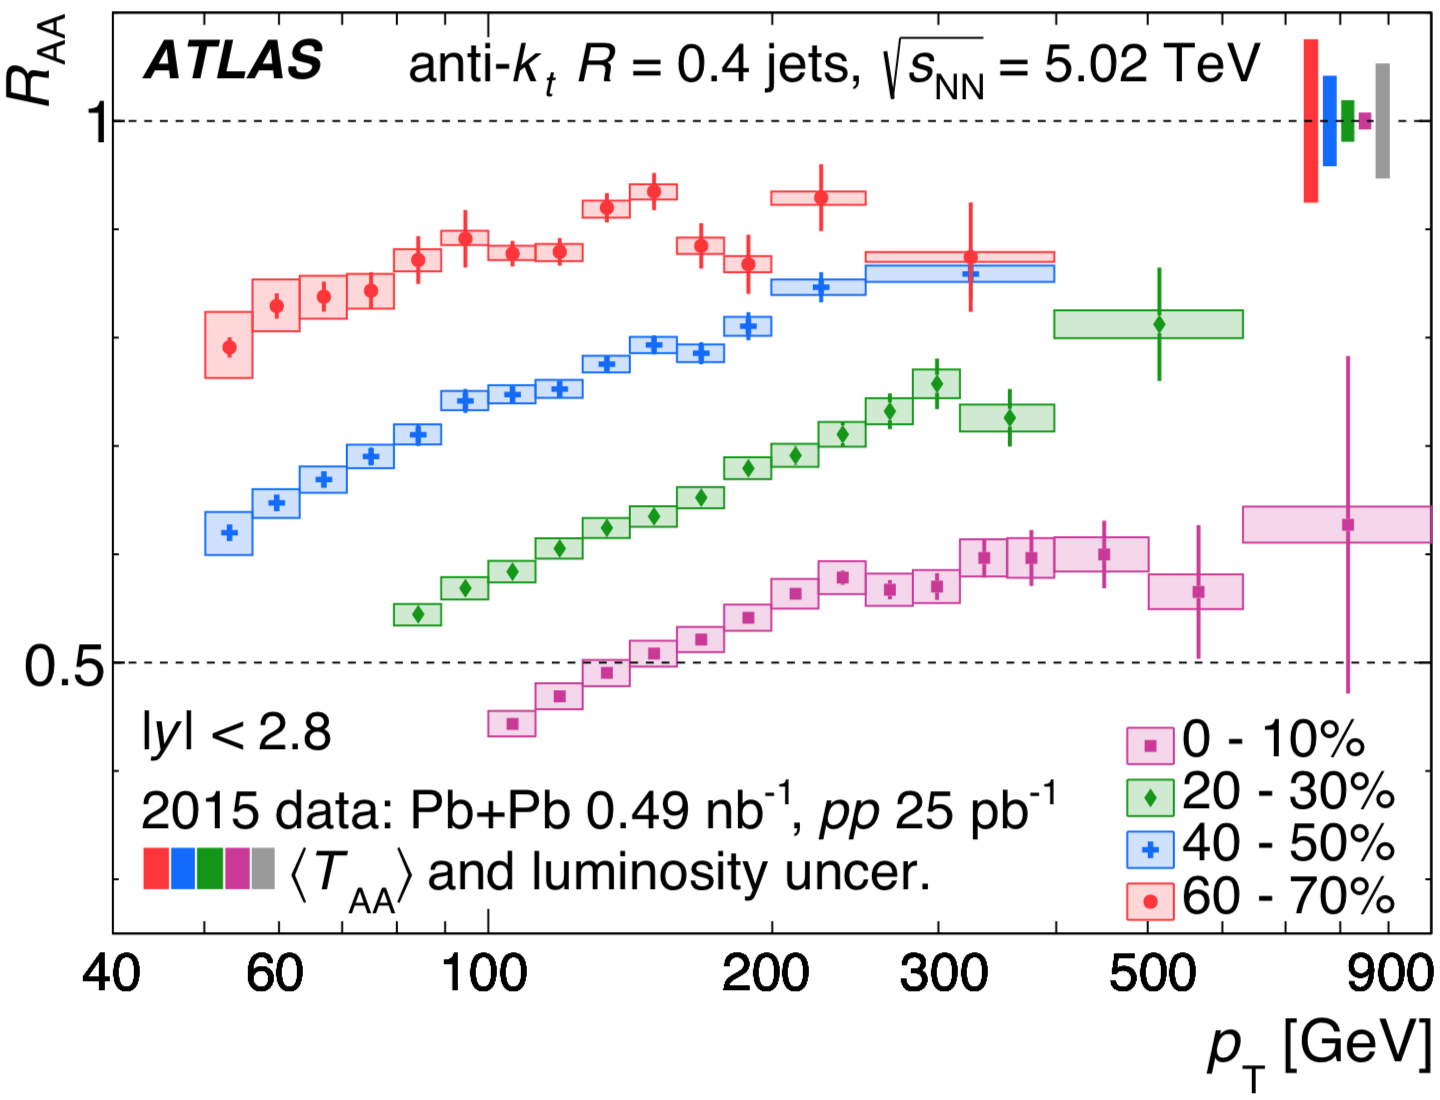
\includegraphics[width=.6\linewidth]{figs/chapter_intro/jet_RAA_ATLAS.png}
\caption{The $R_{AA}$ values as a function of jet $\pT$ for jets with $|y|<2.8$ for four centrality intervals. This figure is taken from Ref.~\cite{Aaboud:2018twu}.}
\label{fig:intro_jet_RAA_ATLAS}
\end{figure}

Another approach to study the effect of jet-medium interaction is the correlated back-to-back jet pairs~\cite{Qin:2015srf}. The energy loss of full jets can be studied by measuring the imbalance/asymmetry of the transverse energies between two correlated jets. The energy asymmetry factor $A_J$ for the correlated jet pairs is defined as:
\begin{equation}
A_J = \frac{E_{\text{T},1}-E_{\text{T},2}}{E_{\text{T},1}+E_{\text{T},2}},
\end{equation}
where $E_{\text{T}, i}$ denotes the transverse energy of the leading and sub-leading jets, respectively. The relative azimuthal angle $\Delta\phi \equiv |\phi_1 - \phi_2|$ between two correlated jets can also provide information about the degree of deflection that jet experience after passing through the hot and dense QGP medium.

The dijet asymmetry and $\Delta\phi$ distributions are shown in four centrality bins in Figure~\ref{fig:intro_jet_asym_ATLAS}, where they are compared with proton-proton data and with fully reconstructed HIJING + PYTHIA simulated events~\cite{Aad:2010bu}. The dijet asymmetry in peripheral Pb+Pb events is similar to that in both $pp$ and simulated events; however, as the events become more central, the Pb+Pb data distributions develop different characteristics, indicating an increased rate of highly asymmetric dijet events. The $\Delta\phi$ distributions show that the leading and second jets are primarily back-to-back in all centrality bins; however, a systematic increase is observed in the rate of second jets at large angles relative to the recoil direction as the events become more central. For a more complete review on jet quenching, refer to Ref.~\cite{dEnterria:2009xfs}.
\begin{figure}[H]
\centering
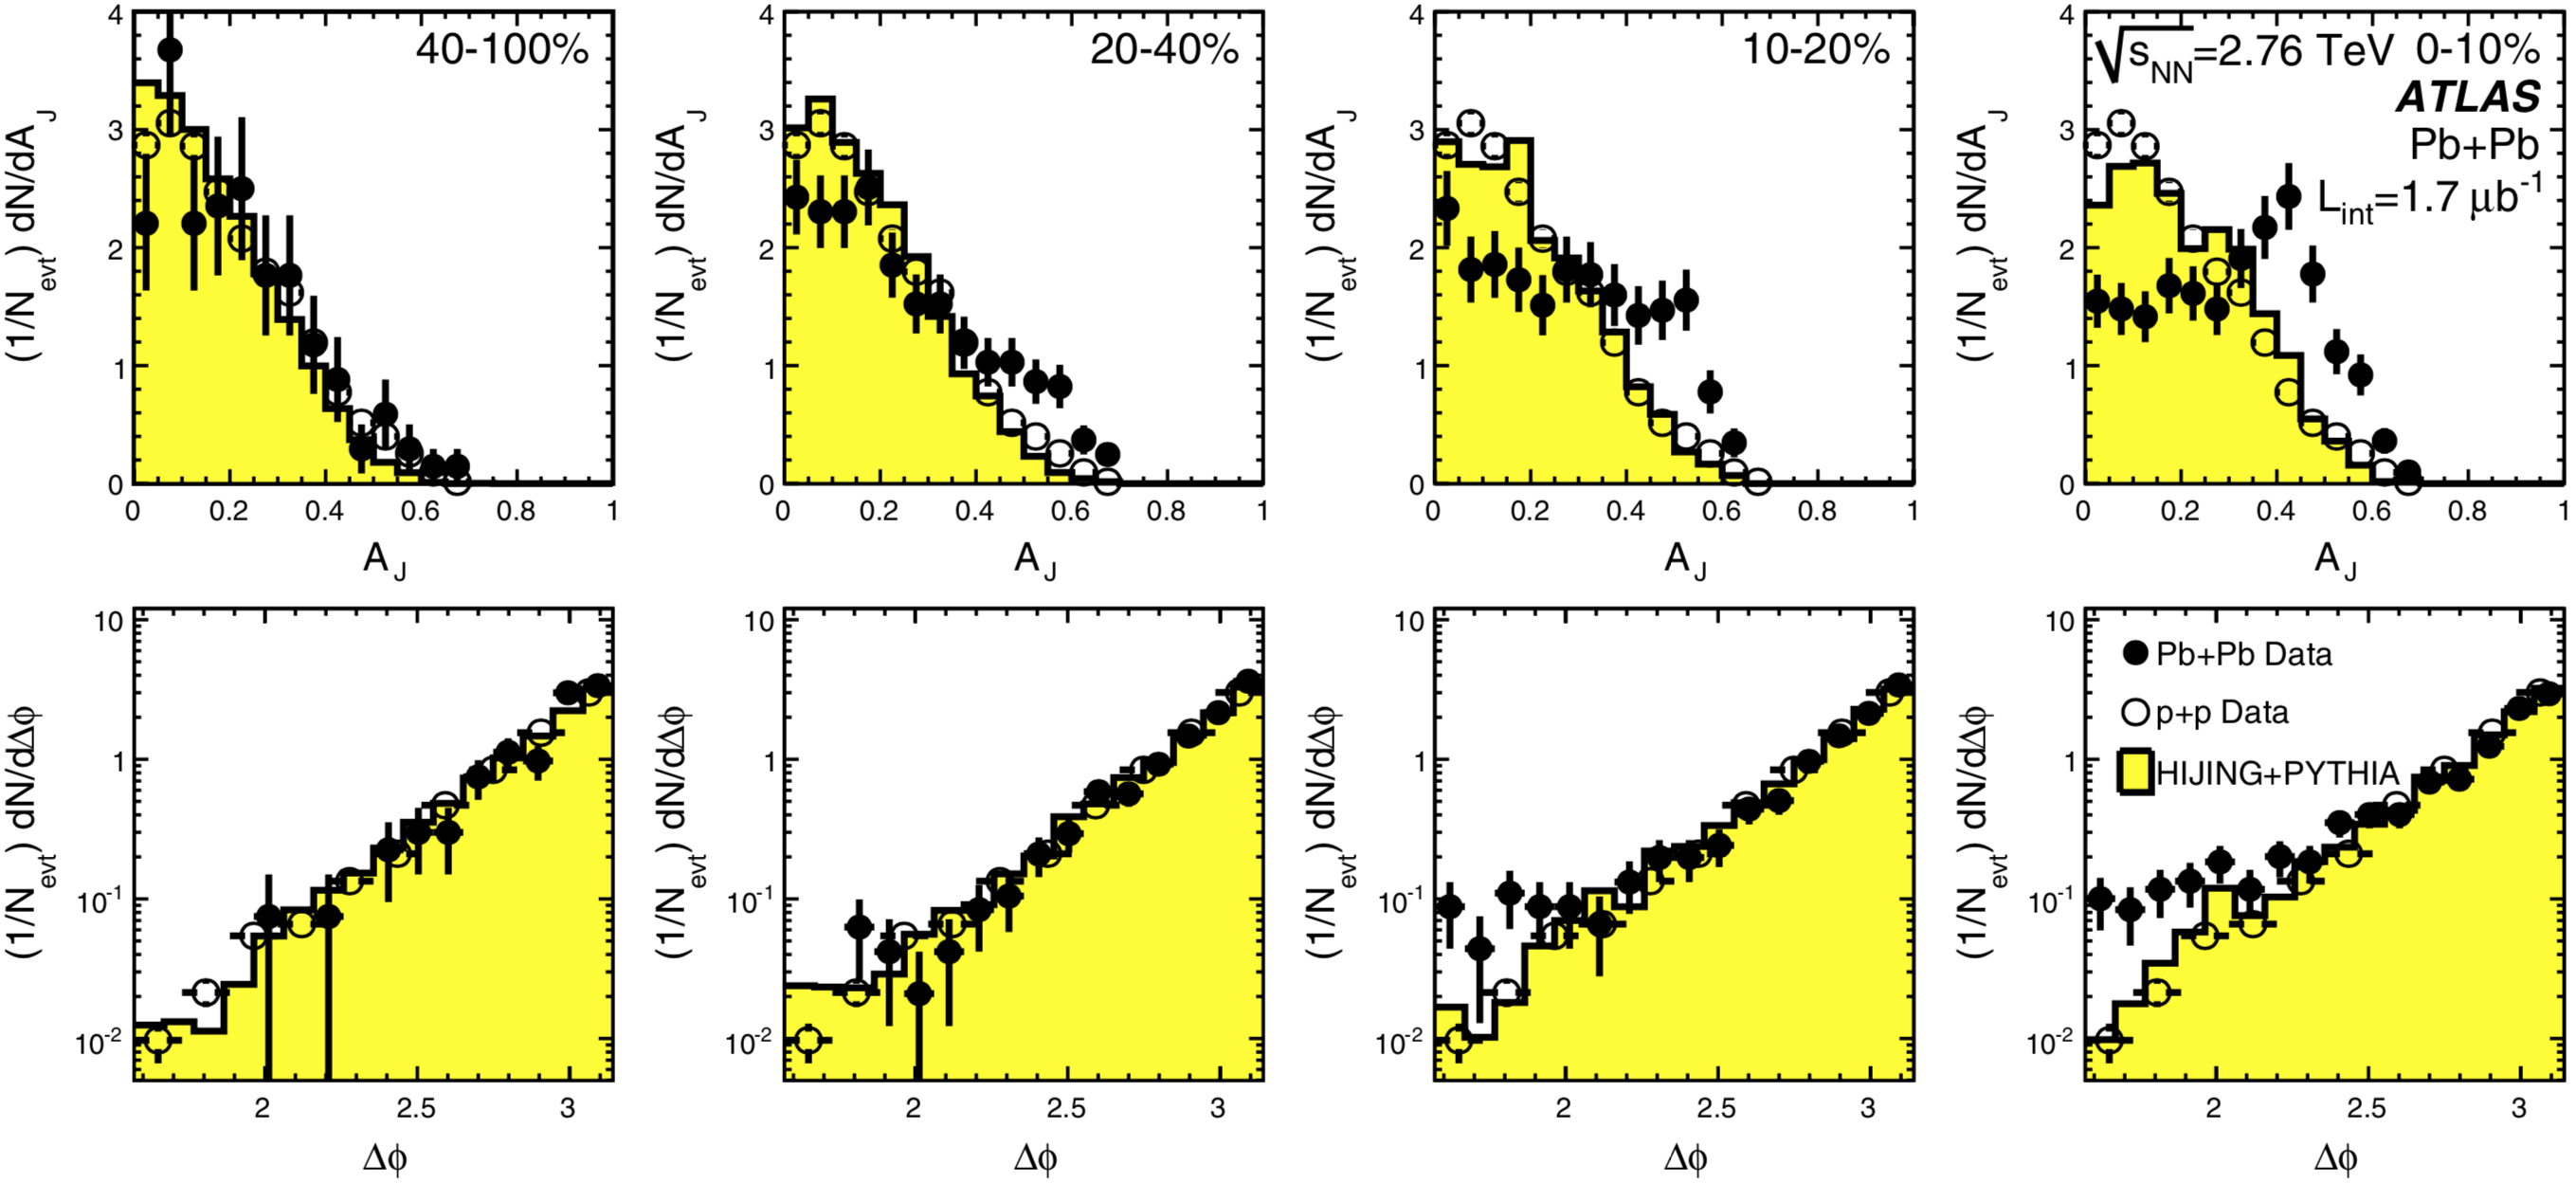
\includegraphics[width=.95\linewidth]{figs/chapter_intro/jet_asym_ATLAS.png}
\caption{Top: dijet asymmetry distribution for data and unquenched HIJING with superimposed PYTHIA dijets, as a function of centrality. Proton-proton data, analyzed with the same jet selection, are shown as open circles. Bottom: Distribution of $\Delta\phi$, the azimuthal angle between the two jets, for data and HIJING + PYTHIA, also as a function of centrality. This figure is taken from Ref.~\cite{Aad:2010bu}.}
\label{fig:intro_jet_asym_ATLAS}
\end{figure}



\subsubsection{Fluctuations of conserved quantities}

Experimental confirmation of the existence of the critical point will be the most direct verification of QCD theory in the non-perturbative region and evidence of the existence of QGP~\cite{Luo:2015cea}. Fluctuations of conserved quantities, such as net-baryon, net-charge and net-strangeness, are predicted to be sensitive to the correlation length of the system~\cite{Stephanov:2008qz} and directly connected to the susceptibilities computed in the theoretical calculations~\cite{Gupta:2011wh}. Thus it can serve as a powerful tool to probe the phase transition and critical point signal in heavy-ion collisions.

Figure~\ref{fig:intro_CP_STAR} shows the energy dependence of $S\sigma$ (ratio of 3rd-order and 2nd-order cumulant) and $\kappa\sigma^2$ (ratio of 4th-order and 2nd-order cumulant) for $\Delta N_p \equiv N_p^+ - N_p^-$ for Au+Au collisions for two collision centralities~\cite{Adamczyk:2013dal}. The $S\sigma$ values normalized to the corresponding Skellam expectations are shown in the bottom panel. The Skellam expectations reflect a system of totally uncorrelated, statistically random particle production. The corresponding results from the $pp$ collisions are also shown and found to be similar to peripheral Au+Au collisions. The data also show deviations from the hadron resonance gas model. The deviations of $S\sigma$ and $\kappa\sigma^2$ below Skellam expectation are qualitatively consistent with a QCD based model which includes a critical point. However the UrQMD model which does not include a critical point also shows deviations from the Skellam expectations. Hence conclusions on the existence of critical point can be made only after multiple sources of backgrounds are removed. For a more complete review of fluctuations of conserved quantities, refer to Ref.~\cite{Luo:2017faz}.
\begin{figure}[H]
\centering
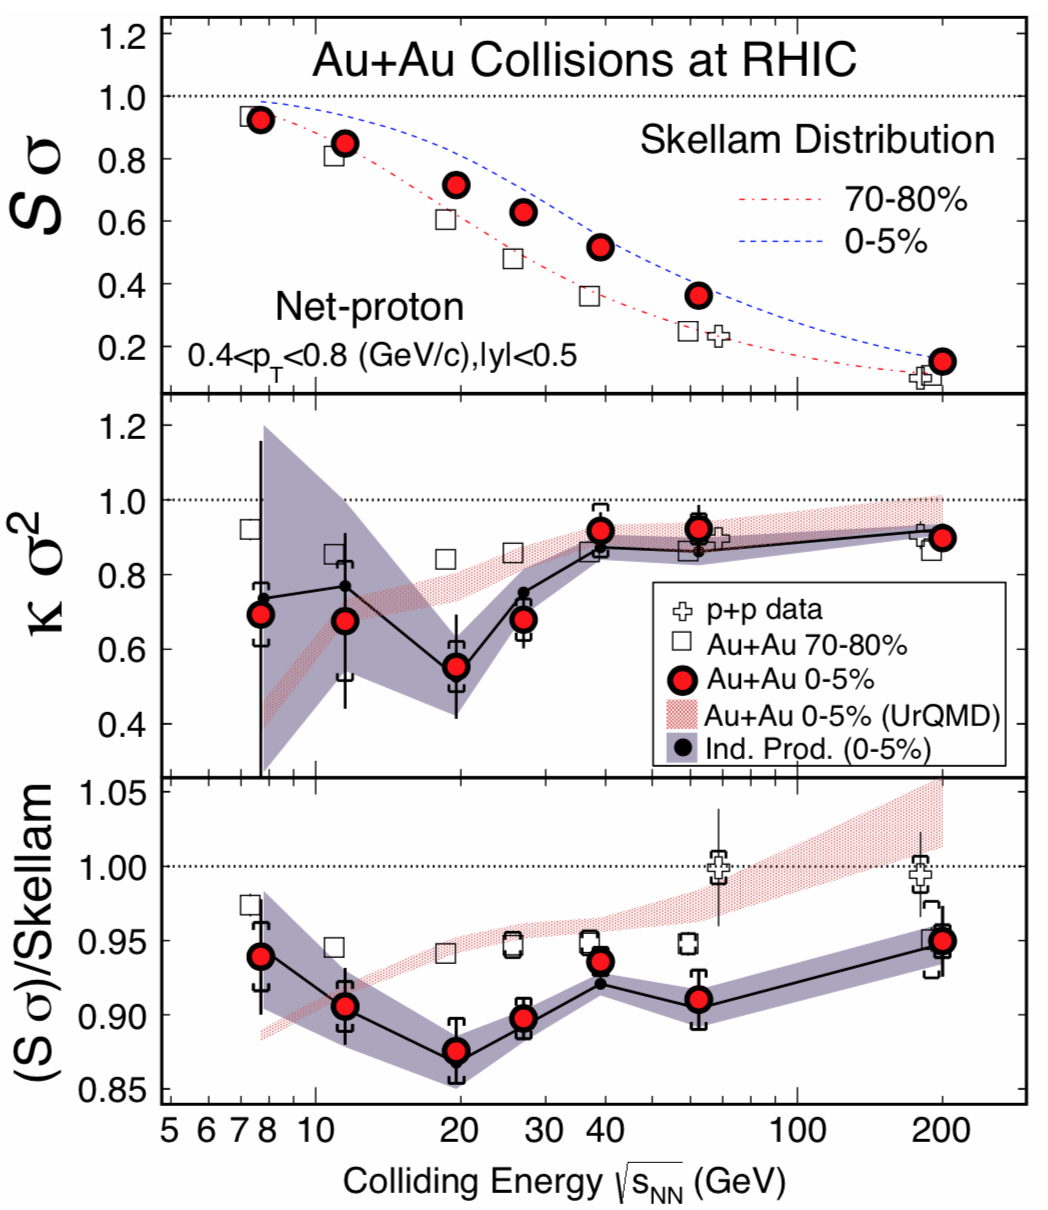
\includegraphics[width=.5\linewidth]{figs/chapter_intro/CP_STAR.png}
\caption{Collision energy and centrality dependence of the net-proton $S\sigma$ and $\kappa\sigma^2$ from Au+Au and $pp$ collisions at RHIC. Skellam distributions for corresponding collision centralities are shown in the top panel. This figure is taken from Ref.~\cite{Adamczyk:2013dal}.}
\label{fig:intro_CP_STAR}
\end{figure}



\subsubsection{Hanbury Brown and Twist (HBT)}

HBT correlations, which probe the space-time extent of a particle-emitting source, may provide valuable insights into the QGP source~\cite{Aaboud:2017xpw}. The HBT method originated in astronomy~\cite{HanburyBrown:1956bqd}, where space-time correlations of photons due to wave function symmetrization are used to measure the size of distant stars. The procedure can be adapted to the extremely small sources encountered in hadronic collisions if identical-particle Bose-Einstein correlations are instead studied in relative momentum space. In a typical HBT analysis, the two-particle correlation functions are fit to a function of relative momentum that is often a Gaussian or exponential function. The parameters of the fits that relate to the space-time extent of the source function are referred to as the HBT radii.

Invariant radii $R_\text{inv}$ are shown for several centralities in Figure~\ref{fig:intro_HBT_ATLAS} as a function a function of the cube root of average $d\Nch / d\eta$~\cite{Aaboud:2017xpw}. For both $k_\text{T}$ intervals shown, the scaling of $R_\text{inv}$ with $\lr{d\Nch / d\eta}^{1/3}$ is close to linear but with a slightly increasing slope at higher multiplicities. This observation is consistent with the prediction that the size of the QGP source should increase with the average multiplicity $d\Nch / d\eta$. In addition, the invariant radius has a steeper trend versus multiplicity at lower $k_\text{T}$. For a more complete review on HBT in heavy-ion collisions, refer to Ref.~\cite{Lisa:2005dd}.

\begin{figure}[H]
\centering
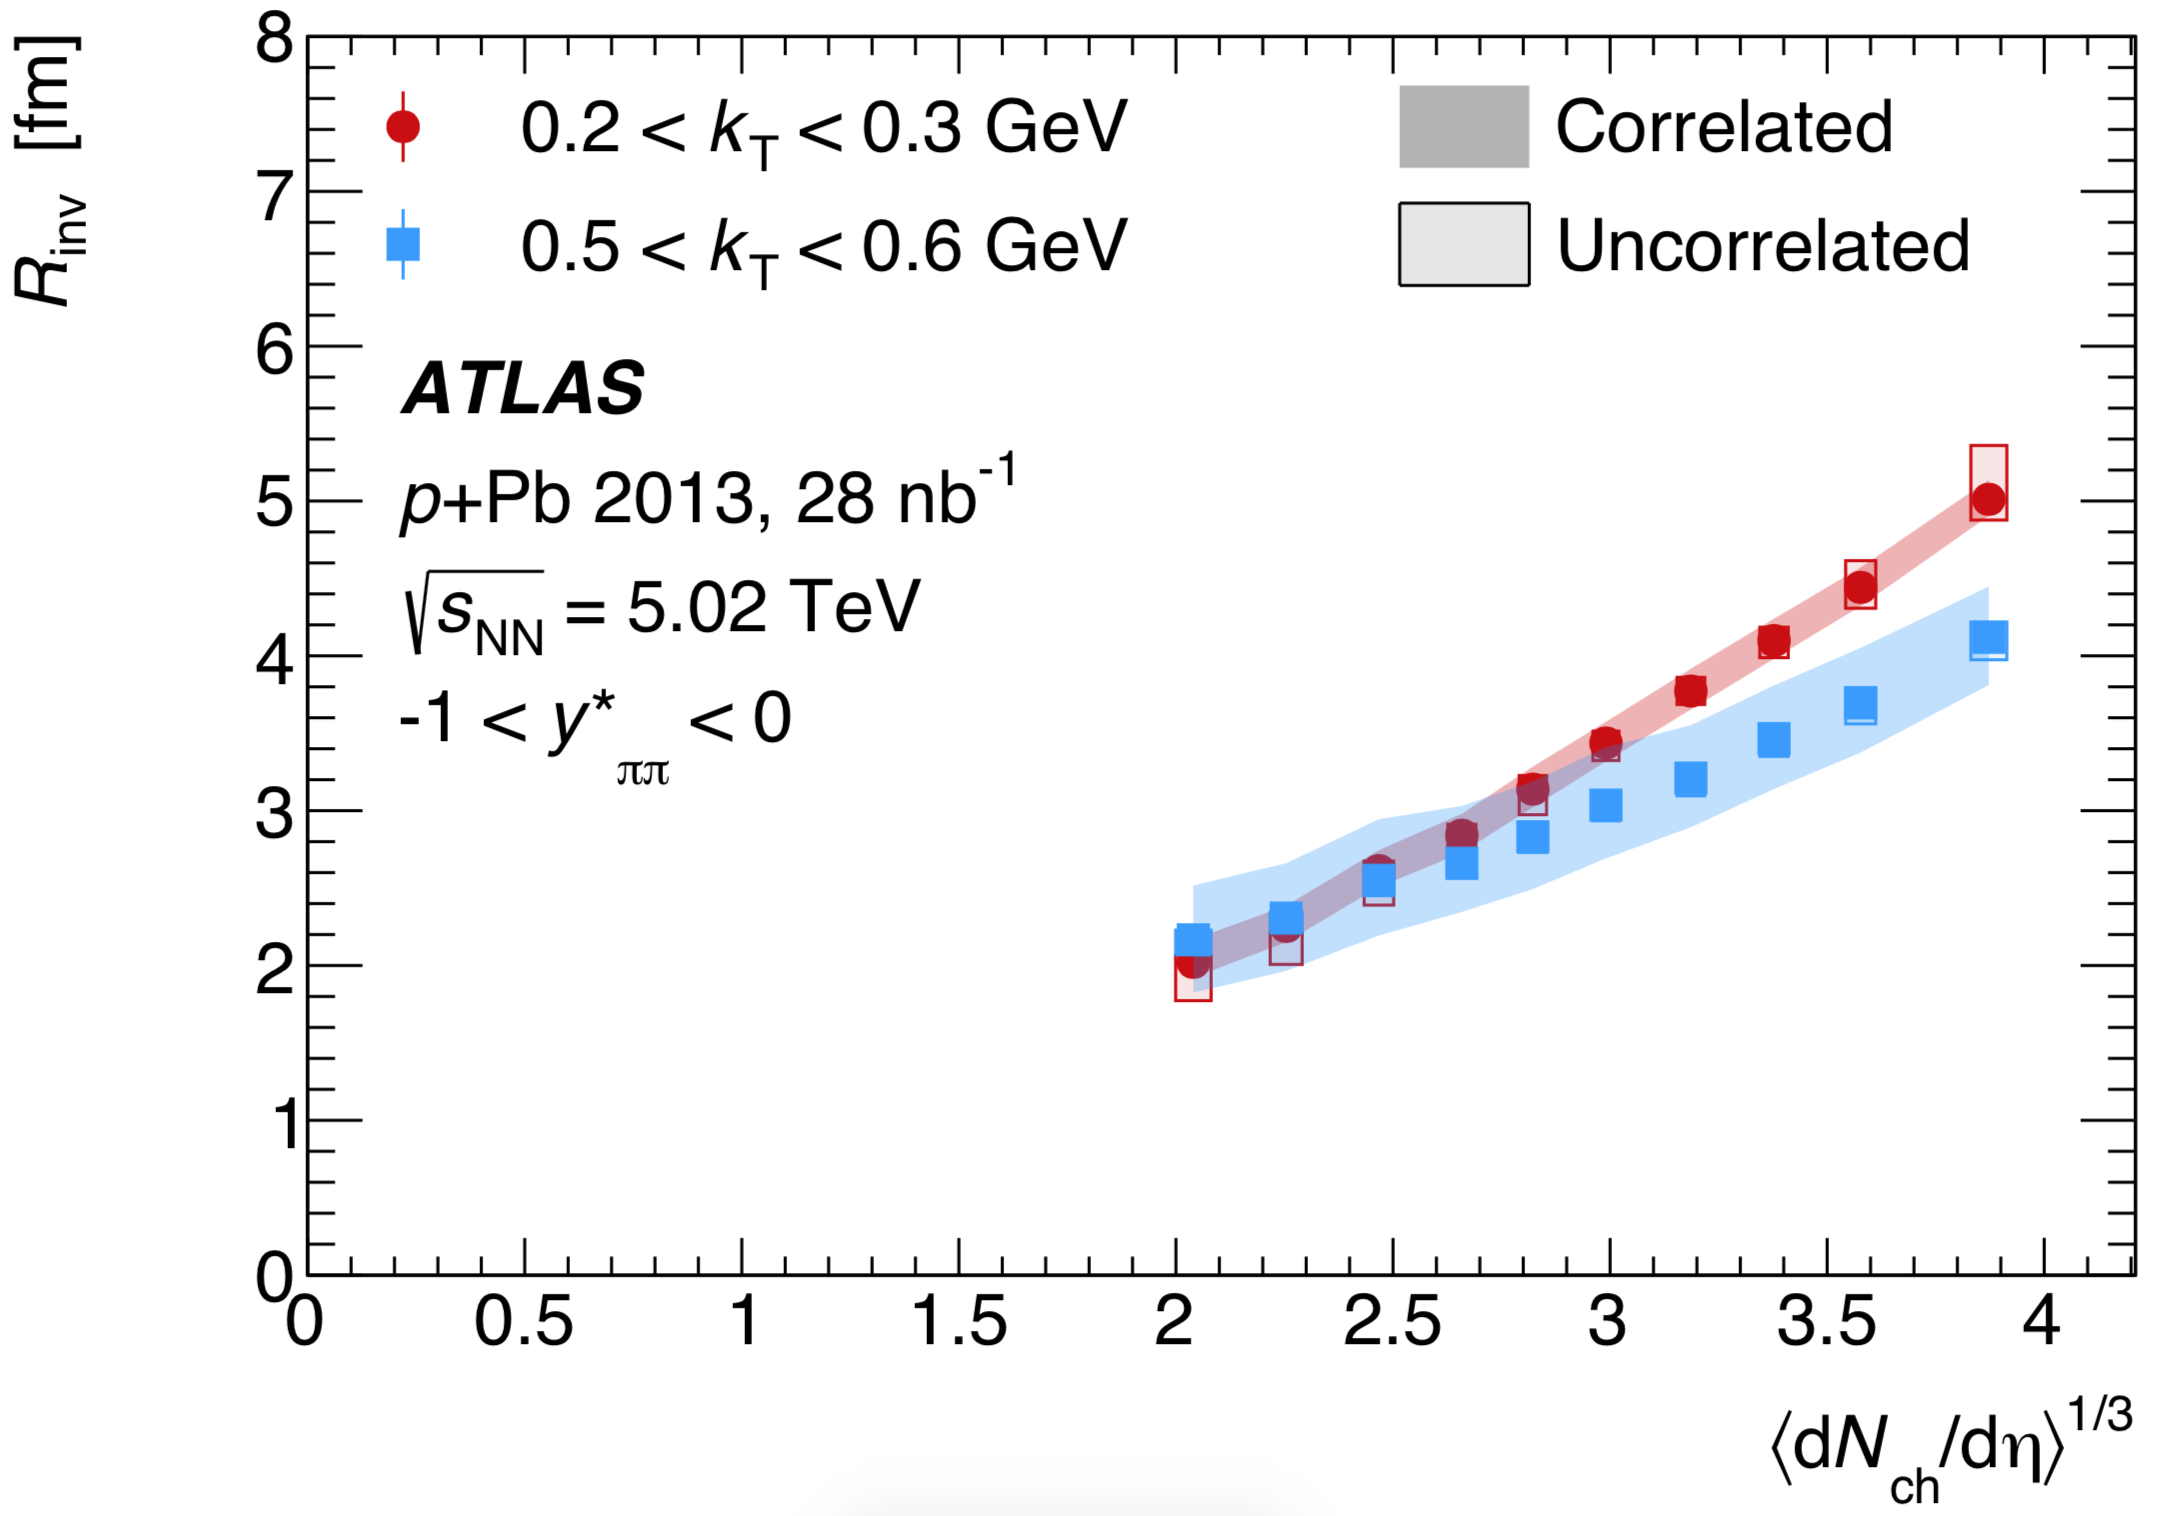
\includegraphics[width=.6\linewidth]{figs/chapter_intro/HBT_ATLAS.png}
\caption{Exponential fit results for Invariant radii $R_\text{inv}$ as a function of the cube root of average charged-particle multiplicity $\lr{d\Nch / d\eta}^{1/3}$, where the average is taken over $|\eta|<1.5$. This figure is taken from Ref.~\cite{Aaboud:2017xpw}.}
\label{fig:intro_HBT_ATLAS}
\end{figure}



\subsection{Motivation of this dissertation}

QGP produced in the HI collisions is unstable and will decay into stable particles that can be observed by detectors. By measuring distribution and event-by-event fluctuation of final stage particles, we could learn the initial stage conditions before the generation of QGP, and the hydrodynamical nature of the QGP expansion. Among all the final stage observables, flow is a fundamental observable to probe the initial spatial anisotropy and the fireball evolution. In this dissertation, we will provide new insights to the current understanding of flow by measuring the multiplicity and flow fluctuation in both transverse and longitudinal directions. In this section, an overview of present status of the flow measurements, as well as the challenges, are presented.



\subsubsection{Measurements in the transverse plane}
\label{sec:transverse_measurements}

The non-uniform initial geometry of the collision zone leads to an azimuthal anisotropy in the profile of the produced particles. The eccentricities in the initial geometry profile would eventually evolve to azimuthal anisotropy for the collision products. Currently there are many aspects of flow measurements in the transverse direction, each trying to address different problems.

\begin{itemize}
\item \textbf{Triangle flow and beyond} In the early days of the flow analysis, due to the "almond-like" shape of the overlap nucleus, elliptic flow ($v_2$) was thought to be dominating the transverse anisotropy. It was later realized that on the event-by-event basis, the initial geometry is not smooth but fluctuates around the average elliptic shape due to random positions of participated nucleons. Triangle flow ($v_3$), and even quadruple flow ($v_4$) provide important constrains on the fluctuations of the initial stage. One challenge in measuring $v_3$ and $v_4$ is that their signal strength are much smaller than the $v_2$. By utilizing the full statistics cumulated over the past few years of LHC, we are able to obtain high precise measurements of $v_3$ and $v_4$ in this dissertation. Refer to Section~\ref{sec:flow_cumulants_for_pvn} for details.
\item \textbf{Correlation between flow harmonics} In the early studies it was regularly assumed that the harmonics $v_n$ respond linearly to the eccentricities $\epsilon_n$ of the same order. However, recent studies argue that a relationship between event-by-event fluctuations of amplitudes of two different flow harmonics $v_n$ and $v_m$ can exist. In this dissertation, we investigated the correlations between $v_2$ and $v_3$, as well as $v_2$ and $v_4$. Refer to Section~\ref{sec:flow_cumulants_for_pvnvm} for details.
\item \textbf{Multi-particle nature of collective flow} An important question about the particle correlation measurements is whether it involves all particles in the event or if it is arises merely from correlations among a few particles. Since collective flow is intrinsically a multi-particle phenomenon, it can be probed more directly using cumulants based on multi-particle correlation techniques. We studied azimuthal correlations involving four and six particles in multiple collision systems. Refer to Section~\ref{sec:flow_cumulants_for_pvn} for details.
\item \textbf{$\pT$ dependence of multi-particle correlations} Another factor that breaks the $v_n \propto \epsilon_n$ is the hydrodynamical evolution and final state effects. Hydrodynamic model calculations suggest strong $\pT$-dependent fluctuations of $v_n$ even in a single event. Such final-state intra-event flow fluctuations may change $v_n$ in a $\pT$ dependent way, and can be quantified by comparing $v_n$ measurements using particles in different $\pT$ ranges. In this dissertation, for each observable, we presented the results in multiple $\pT$ ranges. Refer to Section~\ref{sec:flow_cumulants_for_pvn} for details.
\item \textbf{System size dependence} Experimental data has implied values of $\eta/s$ close to $0.2$ at LHC energy, however, uncertainties in the modeling of the initial state have prevented the extraction of more precision information. The data from different collision systems with different nuclei sizes may provide an opportunity to further constrain $\eta/s$. Our studies utilized the new collected Xe+Xe data, and compared the flow results to previous measured Pb+Pb results. Various initial state models predict Xe+Xe and Pb+Pb collisions have similar values of $\epsilon_2$, therefore the ratios of Xe+Xe to Pb+Pb $v_2$ coefficients in the mid-centrality range could be directly sensitive to $\eta/s$. Refer to Section~\ref{sec:novel_collision_systems_xexe} for details.
\item \textbf{Smallest QGP droplet} Many flow and other measurements have shown that QGP might exist in ion-ion collisions. In recent years, two-particle flow correlation shows hints of elliptic flow in the small systems like proton-proton and proton-lead. To confirm previous observation, we have developed special triggers to collect enough $pp$ events in the high multiplicity region. The four-particle cumulants we measured shows a negative sign that supports the collective phenomenon in the small systems. Our new results contributed to the discussions in search for the smallest QGP droplet produced in the experiment. Refer to Section~\ref{comparison_between_different_cumulant_methods} for details. (For a review of collectivity in small systems, refer to Ref.~\cite{Nagle:2018nvi}.)
\item \textbf{Background suppression} Depending on the signals we are interested in, there are many backgrounds that need to be suppressed. In the flow measurements, one of the most significant background arises from particle correlations among a few particles, due to resonance decays, jets, or multi-jet production (non-flow). Non-flow is especially significant in smaller collision systems and we have developed a novel subevent algorithm to effectively remove such background. Another important background originates from our limited access to the initial stage quantities such as number of participating nucleons $N_\text{part}$. Since centrality defined in experiment is only an estimate of $N_\text{part}$ on the average level, the fluctuation of centrality will have an impact on all the fluctuations measurements. In this dissertation, we also spent some efforts investigating such effect in flow cumulant measurements. Refer to Section~\ref{sec:subevent_cumulant_method} and Section~\ref{sec:glauber_model} for details.
\end{itemize}



\subsubsection{Measurements in the longitudinal direction}

Before the collision of nucleus, the number of nucleon participants in the target and projectile fluctuate from event-to-event. This longitudinal fluctuation directly affects the entropy production at very early time of the collision, well before the onset of the collective flow. Experimental measurements provide a window into the space-time picture of the collective expansion as well as the medium properties that drives the expansion.

Longitudinal correlations have been measured extensively in previous studies, however, many questions still remain to be addressed. There are currently two majors areas for longitudinal measurements:
\begin{itemize}
\item \textbf{Multiplicity correlation} To study the early-time density fluctuations in pseudorapidity, forward-backward correlations of particle multiplicity in two $\eta$ ranges were measured in many collision systems. Instead of using limited information, we proposed a more general and comprehensive method by decomposing the correlation function into orthogonal Legendre polynomial functions (or into principal components as suggested by others), each representing a unique component of the measured forward-backward correlation. Furthermore, we developed a data-driven method to suppress the multiplicity correlations from the final state such as resonance decays, single-jet fragmentation, and Bose-Einstein correlations. In this dissertation, our new methods were applied from large to small collision systems. Refer to Section~\ref{sec:fb_atlas_data} for details.
\item \textbf{Flow decorrelation} Most previous flow studies assumed that the initial condition and space-time evolution of the matter are boost-invariant in the longitudinal direction. Recent model studies of two-particle correlations as a function of pseudorapidity $\eta$ revealed strong event-by-event fluctuations of the flow magnitude and phase between two well-separated pseudorapidities, named as flow decorrelation. Even though in this dissertation we do not measure flow decorrelation directly, we will have brief discussions on this topic when introducing the subevent technique. Refer to Section~\ref{sec:flow_decorrelation} for details.
\end{itemize}



\subsection{Outline of this dissertation}

In the first half of Section~\ref{chapter:detector}, we will introduce the setup of Large Hadron Collider and describe all the sub-detectors of the ATLAS detector that have been used in our measurements. In the second half of Section.~\ref{chapter:detector}, we will explain how the data (Pb+Pb, Xe+Xe, $p$+Pb and $pp$) were gathered and cleaned. Track selection and reconstruction procedures are also discussed in this section.

In Section~\ref{chapter:fbcorr}, we will present the longitudinal multiplicity correlation measurements, using HIJING and AMPT models, as well as the ATLAS data. We will first discuss the limitations of previous analyses, and then introduce a new observable to dissect longitudinal dynamics. A data-driven technique to suppression background is explained. After presenting the results in models and data, we will summarize and discuss the potential improvements on the measurements.

In Section~\ref{chapter:subcumu}, we will present the subevent flow cumulant studies, using PYTHIA model and the ATLAS data. We will first point out that the standard cumulant method suffers from non-flow background, then the state-of-the-art subevent algorithm is introduced and validated in model. After applying the new method successfully to ATLAS data, we will also discuss the extension of this new method to other measurements.

In Section~\ref{chapter:centfluc}, we will present the flow and centrality fluctuation studies, using Glauber model and ATLAS data. First, we will explain what is centrality fluctuation and how to measure it in a simple Glauber model. Then we will explain how to qualitatively measure this effect in a model-independent way. Different collision system, Xe+Xe, will also be covered at the end of this section.

In Section~\ref{chapter:summary}, we will review all the puzzles and challenges we mentioned in the introduction section, then summarize how the studies in this dissertation help to answer those questions.

In the Appendix~\ref{chapter:appendix}, two technical aspects of our studies will be discussed: first is how to develop an algorithm to speed up the multi-particle cumulant calculation; second is a walk-through of estimating the systematic uncertainties in these measurements.











